%%%%%%%%%%%%%%%%%%%%%%% file typeinst.tex %%%%%%%%%%%%%%%%%%%%%%%%%
%
% This is the LaTeX source for the instructions to authors using
% the LaTeX document class 'llncs.cls' for contributions to
% the Lecture Notes in Computer Sciences series.
% http://www.springer.com/lncs       Springer Heidelberg 2006/05/04
%
% It may be used as a template for your own input - copy it
% to a new file with a new name and use it as the basis
% for your article.
%
% NB: the document class 'llncs' has its own and detailed documentation, see
% ftp://ftp.springer.de/data/pubftp/pub/tex/latex/llncs/latex2e/llncsdoc.pdf
%
%%%%%%%%%%%%%%%%%%%%%%%%%%%%%%%%%%%%%%%%%%%%%%%%%%%%%%%%%%%%%%%%%%%


\documentclass[runningheads,a4paper]{llncs}
\usepackage{amssymb}
\setcounter{tocdepth}{3}
\usepackage{graphicx}

\usepackage{url}
\newcommand{\keywords}[1]{\par\addvspace\baselineskip
\noindent\keywordname\enspace\ignorespaces#1}

\begin{document}

\mainmatter  % start of an individual contribution

% first the title is needed
\title{Developing an Ecosystem for Interactive
Electronic Implants}

% a short form should be given in case it is too long for the running head
\titlerunning{Initial Steps in Designing Interactive Electronic Implants}

% the name(s) of the author(s) follow(s) next
%
% NB: Chinese authors should write their first names(s) in front of
% their surnames. This ensures that the names appear correctly in
% the running heads and the author index.
%
\author{anonymized\inst{1}
\and anonymized\inst{2}
\and anonymized\inst{3}}
%
\authorrunning{Initial Steps in Designing Interactive Electronic Implants}
% (feature abused for this document to repeat the title also on left hand pages)

% the affiliations are given next; don't give your e-mail address
% unless you accept that it will be published
\institute{anonymized,
\email{anonymized}\\
\and
anonymized
\email{anonymized}\\
\and
anonymized,
\email{anonymized}}
%
% NB: a more complex sample for affiliations and the mapping to the
% corresponding authors can be found in the file "llncs.dem"
% (search for the string "\mainmatter" where a contribution starts).
% "llncs.dem" accompanies the document class "llncs.cls".
%

\toctitle{Designing an Ecosystem for Interactive
Electronic Implants}
\maketitle


\begin{abstract}

In this work in progress report we present Remora, a system for designing interactive subdermal devices. Remora builds upon methods and technologies developed by body modification artists. The development has so far focussed on battery and power management as well as redundancy features. Remora consists of a series of hardware modules and a corresponding software environment. Remora is designed for body modification artists to design their own implants, but will also be a platform for researchers interested in sub-dermal interaction and hybrid systems. We have so far implemented a prototype device; future work will include in depth evaluation of this device as well as user studies, a graphical development environment and additional hardware and software modules.

\keywords{Implantable Devices, Subcutaneous Interaction, Human-Machine Hybrids}
\end{abstract}


\section{Introduction}
There is growing interest in interacting with devices inside the body in the Human Computer Interaction (HCI) research community, as well as in the Body Modification Community. Implanted devices are anticipated to provide opportunities for sensory augmentation, biometric data collection, data-storage or novel HCI applications [1, 2]. This growing interest can be observed looking at workshops at leading HCI conferences\footnote{https://insertables.wordpress.com/},  various self-experimentation projects, such as the Circadia by Grindhouse Wetware [3], or review papers on this very topic [4].

Implanted devices are not new - pacemakers and dental implants date back to the late 1950’s and have since become established in medical practice. Common medical implants include joint replacements, drug delivery systems, cerebral shunts, stents, cardiac monitors and pacemakers, and even brain implants that provide deep brain stimulation to Parkinson patients or treat seizures for epilepsy patients. Implants are also common for plastic surgery purposes, most notably the breast implant, which dates back to the 1960’s.

In parallel to these more established practices, the body modification community has developed methods, practices and technologies of their own, including the development of subdermal implants. These are usually injection molded silicone objects which are implanted under the skin for aesthetic purposes. The manufacturing process of these subdermal implants allows encapsulating objects inside the implant. This enables implantation of unconventional objects, such as the ashes of a loved one or electronic circuitry. There is a trend amongst self-identified ‘grinders’ or ‘wet-ware hackers’ to appropriate these methods for the design of implantable electronic devices [3, 4]. 


\begin{figure}
 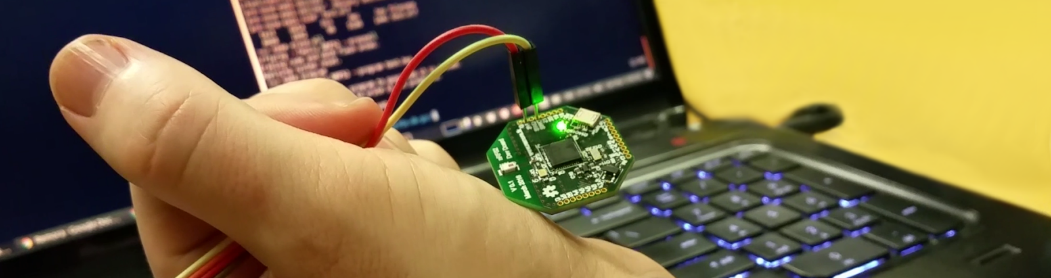
\includegraphics[scale=1]{device}
 

\caption{Remora Prototype}
\end{figure}

Inspired by body modification culture, and in a somewhat worried reaction to the design of devices implanted by ‘grinders’, we are designing Remora (Figure 1), an eco-system for the development of implantable devices. This eco-system conforms to the constraints a body modification artist is faced with when producing and implanting an electronic device. Remora is therefore not intended to improve upon, or even compare to the current state of the art in electronic implantable medical devices. 

Remora aims to provide a platform with multiple failsafe and redundancy mechanisms around which to design interactive, subdermal devices. We anticipate this to find use in the body modification community, however we also believe that various research communities will benefit from such a platform. For example, Remora would allow research into sub-cutanious sensing [1] to progress within living bodies, and enable novel human computer interaction methods, advanced biometric monitoring and research into brain plasticity. 

Remora will consist of a development environment for designing ultra-low power applications, as well as a wireless bootloader with redundancy and self-monitoring functions. This will be paired with hardware module designs which can be combined based on the requirements of a given application. The resulting device would then be encapsulated in parylene C coating and embedded in implant grade silicone. The resulting silicone object can be inserted under the skin using methods established by body modification artists.
 
\section{Related Work}
\subsection{Posthuman Bodies}
Art that challenges the traditional role of the body is becoming succeedingly more mainstream. French artist Orlan has exhibited her plastic surgery performance at the Guggenheim in NYC, while Australian artist Stelarc has become a common reference at human computer interaction conferences. Stelarc's works explore the theme of agency beyond the body. His artworks often involve performances in which control over his limbs is handed to the audience or to random signals generated by internet traffic. He also uses robotic appendixes to expand his body and has experimented with implantation of extra sensory organs [5].

While artists such as Stelarc and Orlan are becoming more mainstream, the body modification community still strongly identifies as a counterculture movement. One of the earliest functional implants common within the body-modification community is a magnet. An implanted magnet vibrates when the implantee is subjected to a varying electromagnetic field. This might occur when walking through security systems or in the close proximity of electric motors or transformers. The first magnetic implants were implanted by Samppa von Cyborg in 2000. 
Kevin Warwick experimented with direct communication between the nervous system of two implantees. He used a 100 pin micro-array as an electrical interface with the nervous system of each implantee. Nervous impulses were then wirelessly transmitted between them. Warwick was also one of the first to implant RFID tags [6]. RFID and NFC implants have been further popularized by Amal Graafstra [7].

The methods developed by the body modification community have recently been appropriated by self identified ‘grinders’, ‘wet-ware-’ or ‘bio hackers’. Most notably Tim Cannon and Grindhouse Wetware have developed a temperature monitoring device and an implantable silicone object illuminated from the inside. While both device types have been implanted, they were since removed due to safety concerns [3].

\subsection{Development Environments}
There is an ever increasing number of ecosystems and dev-boards that support non-experts in the development of digital devices. Most prominent among them Raspberry Pi and Arduino. Neither however meet the ultra-low power requirements and the compact size required of an implanted device. Other interesting systems include the Bluetooth Low Energy (BLE) development boards by RedBearLabs \footnote{http://redbearlab.com/}  or products based on Simblee \footnote{https://www.simblee.com/}. These solutions have relatively low power consumption, but the form-factor of the devices by RedBearLabs and the closed source of the Simblee protocol are also problematic. There are various upcoming development kits based around the new nRF52, such as the BMD-300  by Rigado \footnote{https://www.rigado.com/product/bmd-300/} with even lower power consumption. While such modules have optimized power consumption, they do not provide the close coupling with wireless charging and battery monitoring which we envision.

\section{Design Space}
\subsection{Implantation Style}
Body modification artists typically distinguish between transdermal and subdermal implants. \textbf{Transdermal} implants contain a metal base and a threaded stud extending beyond the skin, on which jewelry - for example metal horns - can be mounted. Depending on the design of the transdermal implant, it might have a porous base which increases the strength with which it is fused to the skin. Transdermals developed by Samppa von Cyborg contain a hydroxyapatite coating to allow it to fuse with human bone. These implants, once healed, are difficult to remove. Transdermal implants also provide an opening in the human body through which bacteria or infections can enter and require continuous care and attention by the implantee. \textbf{Subdermal} implants are placed underneath the skin. As the skin can close above it, such implants minimize the risk of both infection and rejection. As the silicone is smooth without any porous structures for the skin to latch on to, removal of such an implant is comparably simple.
\subsection{Functionality}
We define all implants which do not exhibit any behavior as non-functional (some, such as breast implants, may have social functions, but do not exhibit any behavior of their own, so we consider them non-functional). There are two main types of \textbf{passive implants} which are gaining increasing popularity: NFC/RFID chips and magnets. These implants transmit and ID or alert the implantee of the presence of a varying electromagnetic field respectively, however they require an external power source. In contrast to these are various explorations into \textbf{active powered implants}, most notably the Circadia and North Star by Grindhouse Wetware. While these devices can turn LEDs on and off on demand, or stream temperature data, they have no way of interacting with the implantees body or environment in real time. Remora will support the design of \textbf{interactive implants}: implants which can react to the implantees bodies, environment and activities both continuously and in real time. 



\section{Implementation}
\subsection{Hardware}
Remora consists of a Core and Extensions (Figure 2). The Core includes the Power Transfer Module, the Battery Module, and the Logic Module. Remora’s functionality is determined by the Extension Modules connected to its Core. Such Extension Modules might provide haptic feedback or illuminate the device from the inside. They could collect inertial or biometric data or enable explicit user input. This modular approach was chosen to give developers the greatest possible freedom in developing their own devices. Example devices might include sensory augmentation applications, such as a device which provides a haptic impulse when the implantee is facing north, continuous biometric monitoring, or internal data storage. 

The Core consists of a Logic Module, Power Transfer Module and Battery Module (see Figure 2). Currently we have also implemented an Inertial Sensing Unit as our first Expansion Module.

The \textbf{Battery Module} contains the battery and basic circuitry to protect battery life as well as a kill switch mechanism. When this killswitch is activated all circuits are immediately powered off. The killswitch can be triggered in multiple ways: the user can explicitly activate it, the Battery Module can activate it, if the temperature of the battery or the power consumption exceeds a predetermined threshold, and it can be triggered by the Logic Module, if it detects a problem.
\begin{figure}
 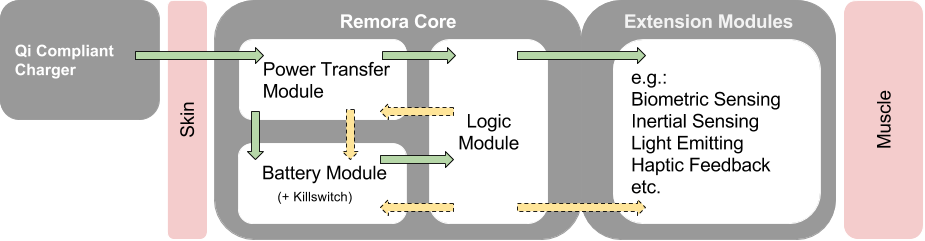
\includegraphics[scale=0.375]{hardware}
 
\caption{Overview of a Remora device. Green solid arrows indicate power flow, yellow dashed arrows indicate control. The Logic Module controls extensions and Battery Module, while the Power Transfer Module only has control over the Battery Module. The Battery Module can be removed completely if one is interested in designing a passive device.}
\end{figure}

For explicit user killswitch activation, we assume that the user has a secondary passive implant consisting solely of a magnet. For example, if the primary implant is in the left arm, the user might have a magnet in the right hand. By touching the magnet of their right hand to the implant in their left hand, the user has a simple and reliable mechanism of disconnecting the battery from the rest of the circuitry.

The \textbf{Power Transfer Module} implements the Qi Compliant Power Transfer standard. This enables users to charge Remora with any off-the-shelf wireless induction charging device. The Qi protocol is implemented using the BQ51050B IC by Texas Instruments. The Power Transfer Module will interrupt the power transfer if: its own temperature rises over a cut-off temperature, if notified of a charging error by the Logic Module, or if it detects the battery to be fully charged. The Qi Compliant standard was chosen because it is currently widely used and therefore a convenient starting point. We anticipate exploring options tailored more specifically to charging an implanted device in the future.

The \textbf{Logic Module} is powered by Nordic Semiconductor's nRF52832. This SoC comes with a Cortex M4 processor and various wireles communication options including NFC and a 2.4GHz radio that supports Bluetooth Low Energy (BLE). The Logic Module supports communication with other devices via UART, SPI and I2C. Additionally the module has a number of GPIOs and 12 bit ADC inputs for interfacing with sensors. The Logic Module monitors its own temperature, the temperature of the Power Transfer Module and the charge state and temperature of the Battery Module. If any of these measures are outside of predetermined levels it can disable wireless charging, activate the killswitch or shut itself down until woken up by explicit user input through the Battery Module.

As any two Core modules can operate with the third module deactivated (See Figure 2), this setup also allows us to collect debug information about the state of the device in case of suspected problems. The Logic Module can be powered from either the Battery Module or the Wireless Power Module and, if intact, provide debug information via Bluetooth. If the Logic Module has failed, battery health information can be extracted from the Power Transfer Model via the Qi communication interface.  

\subsection{Software}
\begin{figure}
 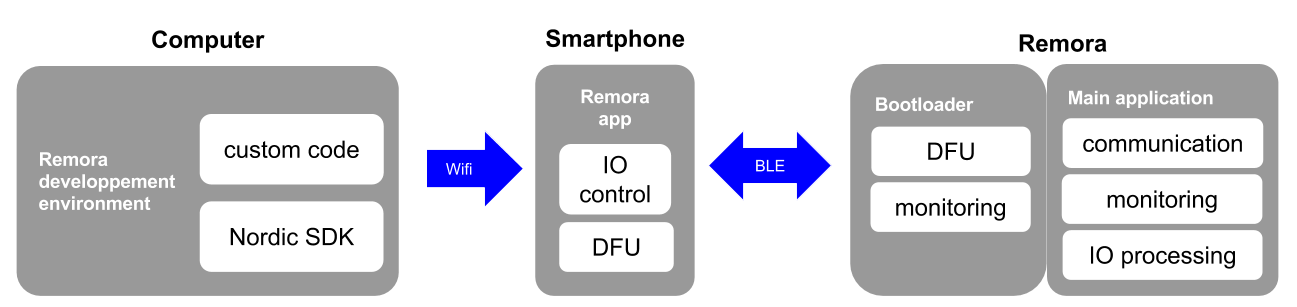
\includegraphics[scale=0.275]{software}
 

\caption{Schematic overview of Remora software architecture}
\end{figure}
The software embedded in the nRF52 consists of two parts, the bootloader and the embedded main application. To develop or customize them, we provide the user with a development environment based on the SDK made by Nordic Semiconductors.

The \textbf{bootloader} performs two functions: it enables firmware uploads using BLE and it takes over monitoring battery health and power consumption, should there be no functioning firmware (Figure 3). The firmware is uploaded using a dual bank memory layout. This ensures that only complete and valid images are activated. During dual bank upload the received firmware is stored in an intermediary memory location and, after it has been fully uploaded and verified, is transferred to its intended location. If an error occurs during the transfer, or if the system is unable to validate the new firmware, the previously uploaded firmware continues operating. The bootloader can be triggered through a BLE request, or by activating the killswitch. 

The \textbf{main application} has several tasks, monitoring \& redundancy, communication and IO processing. The monitoring \& redundancy task is not designed to be modified by the user. It continuously monitors temperature of all modules as well as power drain and battery health. For reliability purpose, these measures are also performed in parallel by dedicated analog circuitry. If either the monitoring \& redundancy task or the analog circuitry determines values to be outside of a predetermined range, the killswitch of the Battery Module is activated. The monitoring \& redundancy task also uses a watchdog monitoring system to restart the processor, should a software endless loop problem occur. Button-less Device Firmware Update (DFU) is conducted using BLE. BLE is also used to provide actuators with external control signals, or send sensor data to other BLE devices. The IO processing is the most modular part and is designed to be completely customizable. It handles communication with extension modules and runs the user created application. 

The development environment is built on top of the development kit provided by Nordic Semiconductors. Users can create custom application using command line arguments and a Makefile, enabling desired extension modules. The development environment optimizes power consumption and memory usage for a given application. It also generates a checksum to avoid transmission errors during the firmware update. Error verification is then performed by the dual bank bootloader. The development environment outputs a zip archive including all required binaries. The archive can then be stored in a cloud services such as Dropbox, to access it from a smartphone app. The smartphone then uploads the firmware using BLE.
\section{Future Work}
We have implemented the three core modules and the inertial sensing module. We have tested these for basic functionality. Our next steps are to add additional hardware modules and to thoroughly evaluate the existing ones. We intend to optimize power consumption using the Simplicity EnergyAware Profiler at body temperature as well as optimize heat-dissipation using a near infrared camera by Optris \footnote{http://silabs.com, http://optris.com}. An open question is which battery technology the final platform should target. Using traditional implantable batteries might not be ideal as our power consumption and charging behaviors are different from existing devices. We wish to emphasize that, as we have not conducted any formal evaluation, we are currently not able to make any statement regarding the safety of our approach.

\section{Conclusion}
In this work in progress report, we presented Remora, an ecosystem for designing implantable devices. Rather than adding to the tradition of mainstream implantable devices, Remora builds on knowledge and practices collected by body modification artists. Remora is designed for these artists to create their own implants, but will also be a platform for researchers interested in creating hybrid systems. Our design is primarily focused on providing series of monitoring and redundancy features, aimed at protecting the implantee and providing the designer with as much debug information as possible, should an error occur. We have so far designed and implemented a proof-of concept device. Future work will expand upon these and include empirical studies testing the safety and reliability of our designs and evaluating interaction design with and for implanted devices.

\section{References}
\begin{enumerate}
  \item Holz, C., Grossman, T.,  Fitzmaurice, G.,  Agur A.: Implanted user interfaces. Proceedings of the 2012 ACM annual conference on Human Factors in Computing Systems (2012) 
  \item Hameed, J.,  Harrison, I.,  Gasson, M.N.,  Warwick, K.:  A novel human-machine interface using subdermal magnetic implants. 2010 IEEE 9th International Conference on Cyberntic Intelligent Systems (2010) 
  \item The Half Life of Body Hacking | Motherboard.\\ http://motherboard.vice.com/read/the-half-life-of-body-hacking.\\ Accessed 20 Mar 2016
  \item Heffernan, K.J.,  Vetere, F.:  You Put What, Where ? Hobbyist Use of Insertable Devices.  Proceedings of the 2016 ACM annual conference on Human Factors in Computing Systems (2016)
  \item	Ping Body - Institute for the Unstable Media. http://v2.nl/events/ping-body. Accessed 21 Oct 2015
  \item	Warwick, K.,  Ruiz V On: linking human and machine brains. Neurocomputing  (2008) 
  \item Graafstra, A.:   Hands On: How radio-frequency identifion and I got personal. IEEE Spectrum 18 23 (2007)

\end{enumerate}





\end{document}
